The Collaborative Memory Network is a CF method and an extensions of NCF \cite{he2017neural} that tries to introduce 
localized user-item interactions using a neighborhood based approach by reweighting with an attention mechanism.
It contains three so called ``memory'' states, a user-, item-and a collective neighborhood memory-state:
Let $\idxi$ corresponds to the one-hot encoded item and $\idxu$ to the one-hot encoded user the user and item memory states are then defined by:
\begin{align*}
  \vec{m}_{\idxu}=\vec{M}\vec{\idxu}&&\vec{e}_{\idxi}=\vec{E}\vec{\idxi}&&\text{with}&&
   \begin{aligned}
    &\vec{\idxi}:=\unitVector_{\idxi}&&\vec{M}\in\R^{P\times d}\\[-1\jot]
    &\vec{\idxu}:=\unitVector_{\idxu}&&\vec{E}\in\R^{Q\times d}
   \end{aligned}                                                                         
\end{align*}
\imp{Output Model:}
the attention mechanism allows to put attention on specific users withing the neighborhood that are similar to the current user of interest.
This weighting can be defined by calculating a user-preference vector $\vec{q}_{\idxu\idxi}$, where each dimension $v$ corresponds to
the endorsement of usre $v$ for item $\idxi$ plus the similarity with the target user $\idxu$: 
\begin{align*}
  \vec{q}_{\idxu\idxi v}&=\vec{m}_{\idxu}^{\T}\vec{m}_{v}+\vec{e}_{\idxi}^{\T}\vec{m}_{v} \qquad\forall v\in N(\idxi)
\end{align*}
the final weighting is then calculated by taking the softmax:\hfil$\vec{p}_{\idxu\idxi v}=\text{softmax}(\vec{q}_{\idxu\idxi v})$\\
This weighting is then used in order to calculate the collective neighborhood memory-state
\begin{align*}
  \vec{o}_{\idxu\idxi}=\sum_{\forall v\in N(\idxi)}\vec{p}_{\idxu\idxi v}\vec{c}_{v}&&\vec{c}_{\idxu}:=\vec{C}\idxu&&\vec{C}\in\R^{P\times d}
\end{align*}
The output/rating $\hat{r}_{\idxu\idxi}$ of the model for a given user and item is then given by:
\begin{align}
  &\vec{z}_{\idxu\idxi}=a_{out}\big(\overbrace{\vec{U}(\vec{m}_{\idxu}\odot\vec{e}_{\idxi})}^{\mathclap{\text{global use-item interaction}}}
  +\underbrace{\vec{W}\vec{o}_{\idxu\idxi}}_{\mathclap{\text{localized user-item-interactions}}}+\vec{b}\big)\quad\xrightarrow{\text{rating}}
  \hat{r}_{\idxu\idxi}=\vec{v}^{\T}\vec{z}_{\idxu\idxi}\nonumber \\[-1\jot]
  &\text{$W,U\in\R^{d\times d},v,b\in\R^d$ are trainable parameters.}
\end{align}
It can be seen that the GMF model \cref{eq:gmf} can be recovered by removing $U$ and the localized interaction.
\begin{figure}[h]
  \centering
  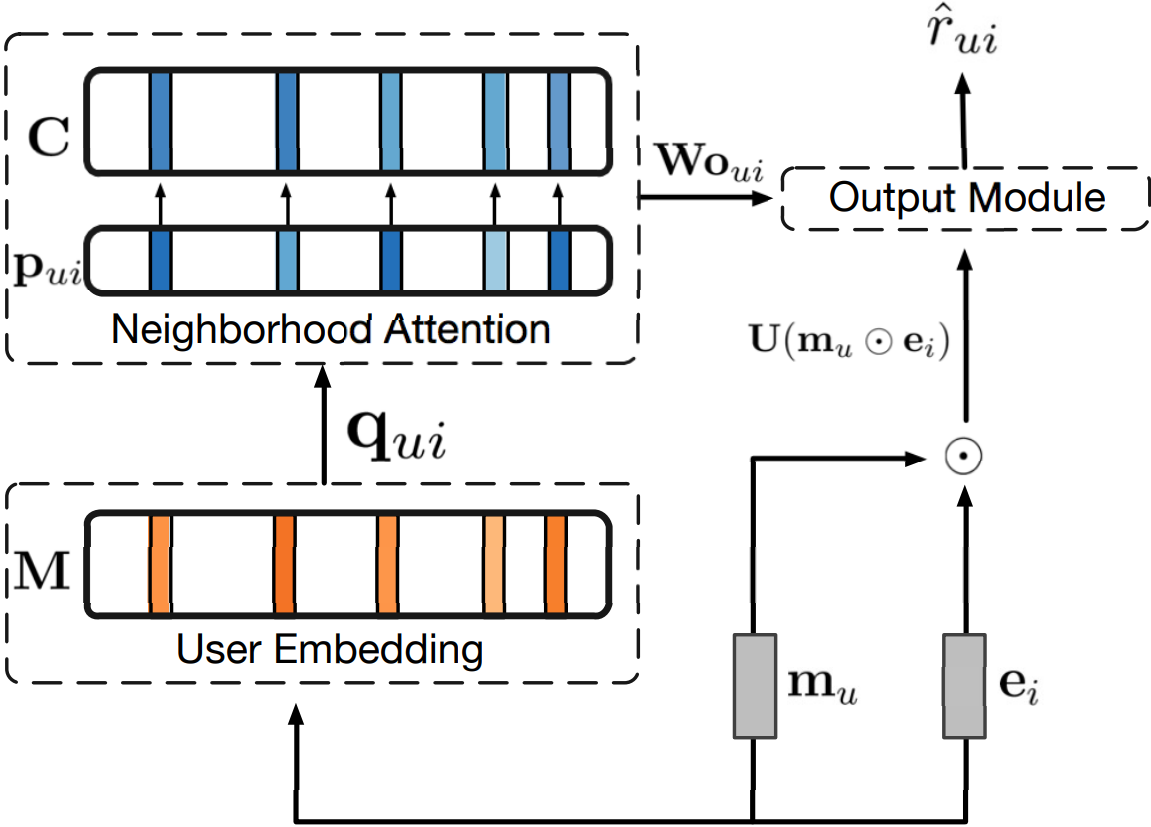
\includegraphics[width=0.7\linewidth]{figures/CMN.png}
  \caption{Schematic of the architecture taken from \cite{he2017neural}}
  \label{fig:}
\end{figure}\\
\imp{Multi-Hop Model:}
multiple of the memory models may be stacked together in order to improve the models predictability:
\begin{align}
  \vec{z}_{\idxu\idxi}^{t}=a_{out}\big(\vec{W}\vec{z}_{\idxu\idxi}^{t-1}+\vec{o}_{\idxu\idxi}^{t}
  +\vec{\mcb}^{t}\big)&&\text{with}&&\vec{z}_{\idxu\idxi}^{0}=\vec{m}_{\idxu}+\vec{e}_{\idxi}
\end{align}
As a loss function the Bayesian Personalized Ranking (BPR) loss was used.
%%% Local Variables:
%%% mode: latex
%%% TeX-master: "../../report"
%%% End:
